\documentclass[10pt]{article}
\usepackage[utf8]{inputenc}


% Set page margins
\usepackage[total={6in,9in}]{geometry}
\usepackage{pdflscape}

% Math packages
\usepackage{amsmath,amssymb}

% Argmin operator
\DeclareMathOperator*{\argmax}{arg\,max}
\DeclareMathOperator*{\argmin}{arg\,min}

% For symbolic footnotes
\usepackage[symbol]{footmisc}

\usepackage{float}
\usepackage{graphicx}
\usepackage{caption}
\usepackage{subcaption}
\usepackage{sidecap} % for side captions
\usepackage{tabu} % for tables
% \usepackage{cleveref} % for referencing multiple equations
\newcommand{\crefrangeconjunction}{--}
\usepackage{array}
\usepackage{tabularx}
\usepackage{booktabs}
\usepackage{siunitx}
\newcolumntype{L}[1]{{\raggedright\arraybackslash}p{#1}}
\usepackage{setspace}

% Packages for table
\usepackage{tabularx}
\usepackage{multirow}
\usepackage{multicol}


% For colourful links
\usepackage{hyperref}
\hypersetup{
    colorlinks=true,
    linkcolor=blue,
    filecolor=magenta,      
    urlcolor=cyan,
    citecolor=blue
}


% Paragraph indentation (none)
\setlength{\parindent}{0pt}
% Paragraph spacing
\setlength{\parskip}{1em}

% boxed equations
\usepackage{empheq}
\usepackage[most]{tcolorbox}
\newtcbox{\mymath}[1][]{%
    nobeforeafter, 
    colframe=black!30!black,
    boxrule=1pt,
    #1}


% Citation superscript
\usepackage[superscript,biblabel]{cite}
\usepackage[super]{natbib}

% Bold the 'Figure #' in the caption and separate it from the title/caption with a period

% Captions will be left justified
\usepackage[aboveskip=1pt,labelfont=bf,labelsep=period,justification=raggedright,singlelinecheck=off]{caption}
\renewcommand{\figurename}{Supplementary Figure}



% Declare operators within the math env
\DeclareMathOperator*{\E}{\mathbb{E}}
\DeclareMathOperator*{\Var}{\text{Var}}
\DeclareMathOperator*{\Tr}{\text{Tr}}
\DeclareMathOperator*{\Det}{\text{Det}}


% Shorthand notation
\newcommand{\smax}{S_{\text{max}}}
\newcommand{\whopf}{w_{\text{Hopf}}}
\newcommand{\wfold}{w_{\text{Fold}}}
\newcommand{\wnull}{w_{\text{Null}}}




% Leave date blank
\date{}

% File path for graphics
\graphicspath{
  {"../figures/"}
}


%--------END MACROS SECTION---------------%


\begin{document}


\section{Empirical predator-prey system}

We test the spectral EWS on data from an empirical predator-prey system that was set up an analysed by Fussmann and colleagues\cite{fussmann00}, which possesses both Hopf bifurcations and a Transcritical bifurcation.

\subsection{Experimental and model overview}

In the study, the authors examined the dynamical behaviour of an aquatic predator-prey system under various nutrient levels, which they regulated via a dilution rate ($\delta$). They found the system exhibited a range of dynamic behaviour including cycles, equilibria of coexistence, and equilibria of extinction, as can be seen in the output time-series of the experiments in Figure \ref{fig:fussmann_tseries}. This behaviour was found to be consistent with a simple mathematical model that captures the fundamental population processes, given by
\begin{align}
    \frac{dN}{dt} & = \delta(N_i - N) - F_C(N) \label{eq:pp1}\\
    \frac{dC}{dt} & = F_C(N) C - F_B(C) B/\epsilon - \delta C \label{eq:pp2}\\
    \frac{dR}{dt} & = F_B(C) R - (\delta + m + \lambda) R \label{eq:pp3}\\
    \frac{dB}{dt} & = F_B(C) R - (\delta + m) B \label{eq:pp4}
\end{align}
where
\begin{equation}
    F_C(N)= \frac{b_C N}{K_C + N}, \quad F_B(C) = \frac{b_B C}{K_B + C}.
\end{equation}
In the model $N$ is the concentration of nitrogen (nutrient), $C$ the concentration of \textit{Chlorella} (prey), $R$ the concentration of reproducing \textit{Brachionus} (predator), and $B$ is the total concentration of $\textit{Brachionus}$. The authors derived parameter values from their own chemostat experiments and published sources of the two species. We use the same parameter values in our study (Table \ref{tab:fussmann_pars}). The conversion factors $\eta_C$ and $\eta_B$ are required to make the units of the model and experimental output consistent. We recreated the bifurcation diagram using the XPPAUT software\cite{ermentrout02} in Figure $\ref{fig:fussmann_ews_pspecs}$a, which shows the different dynamic regimes seperated by three Hopf bifurcations (H1, H2, H3) and a transcritical bifurcation (T1). In what follows, we analyse the standard and spectral EWS in model simulations and experimental output, to validate and test the limitations of the theory.


% Figure: Fussmann time-series
\begin{figure}[H]
\centering
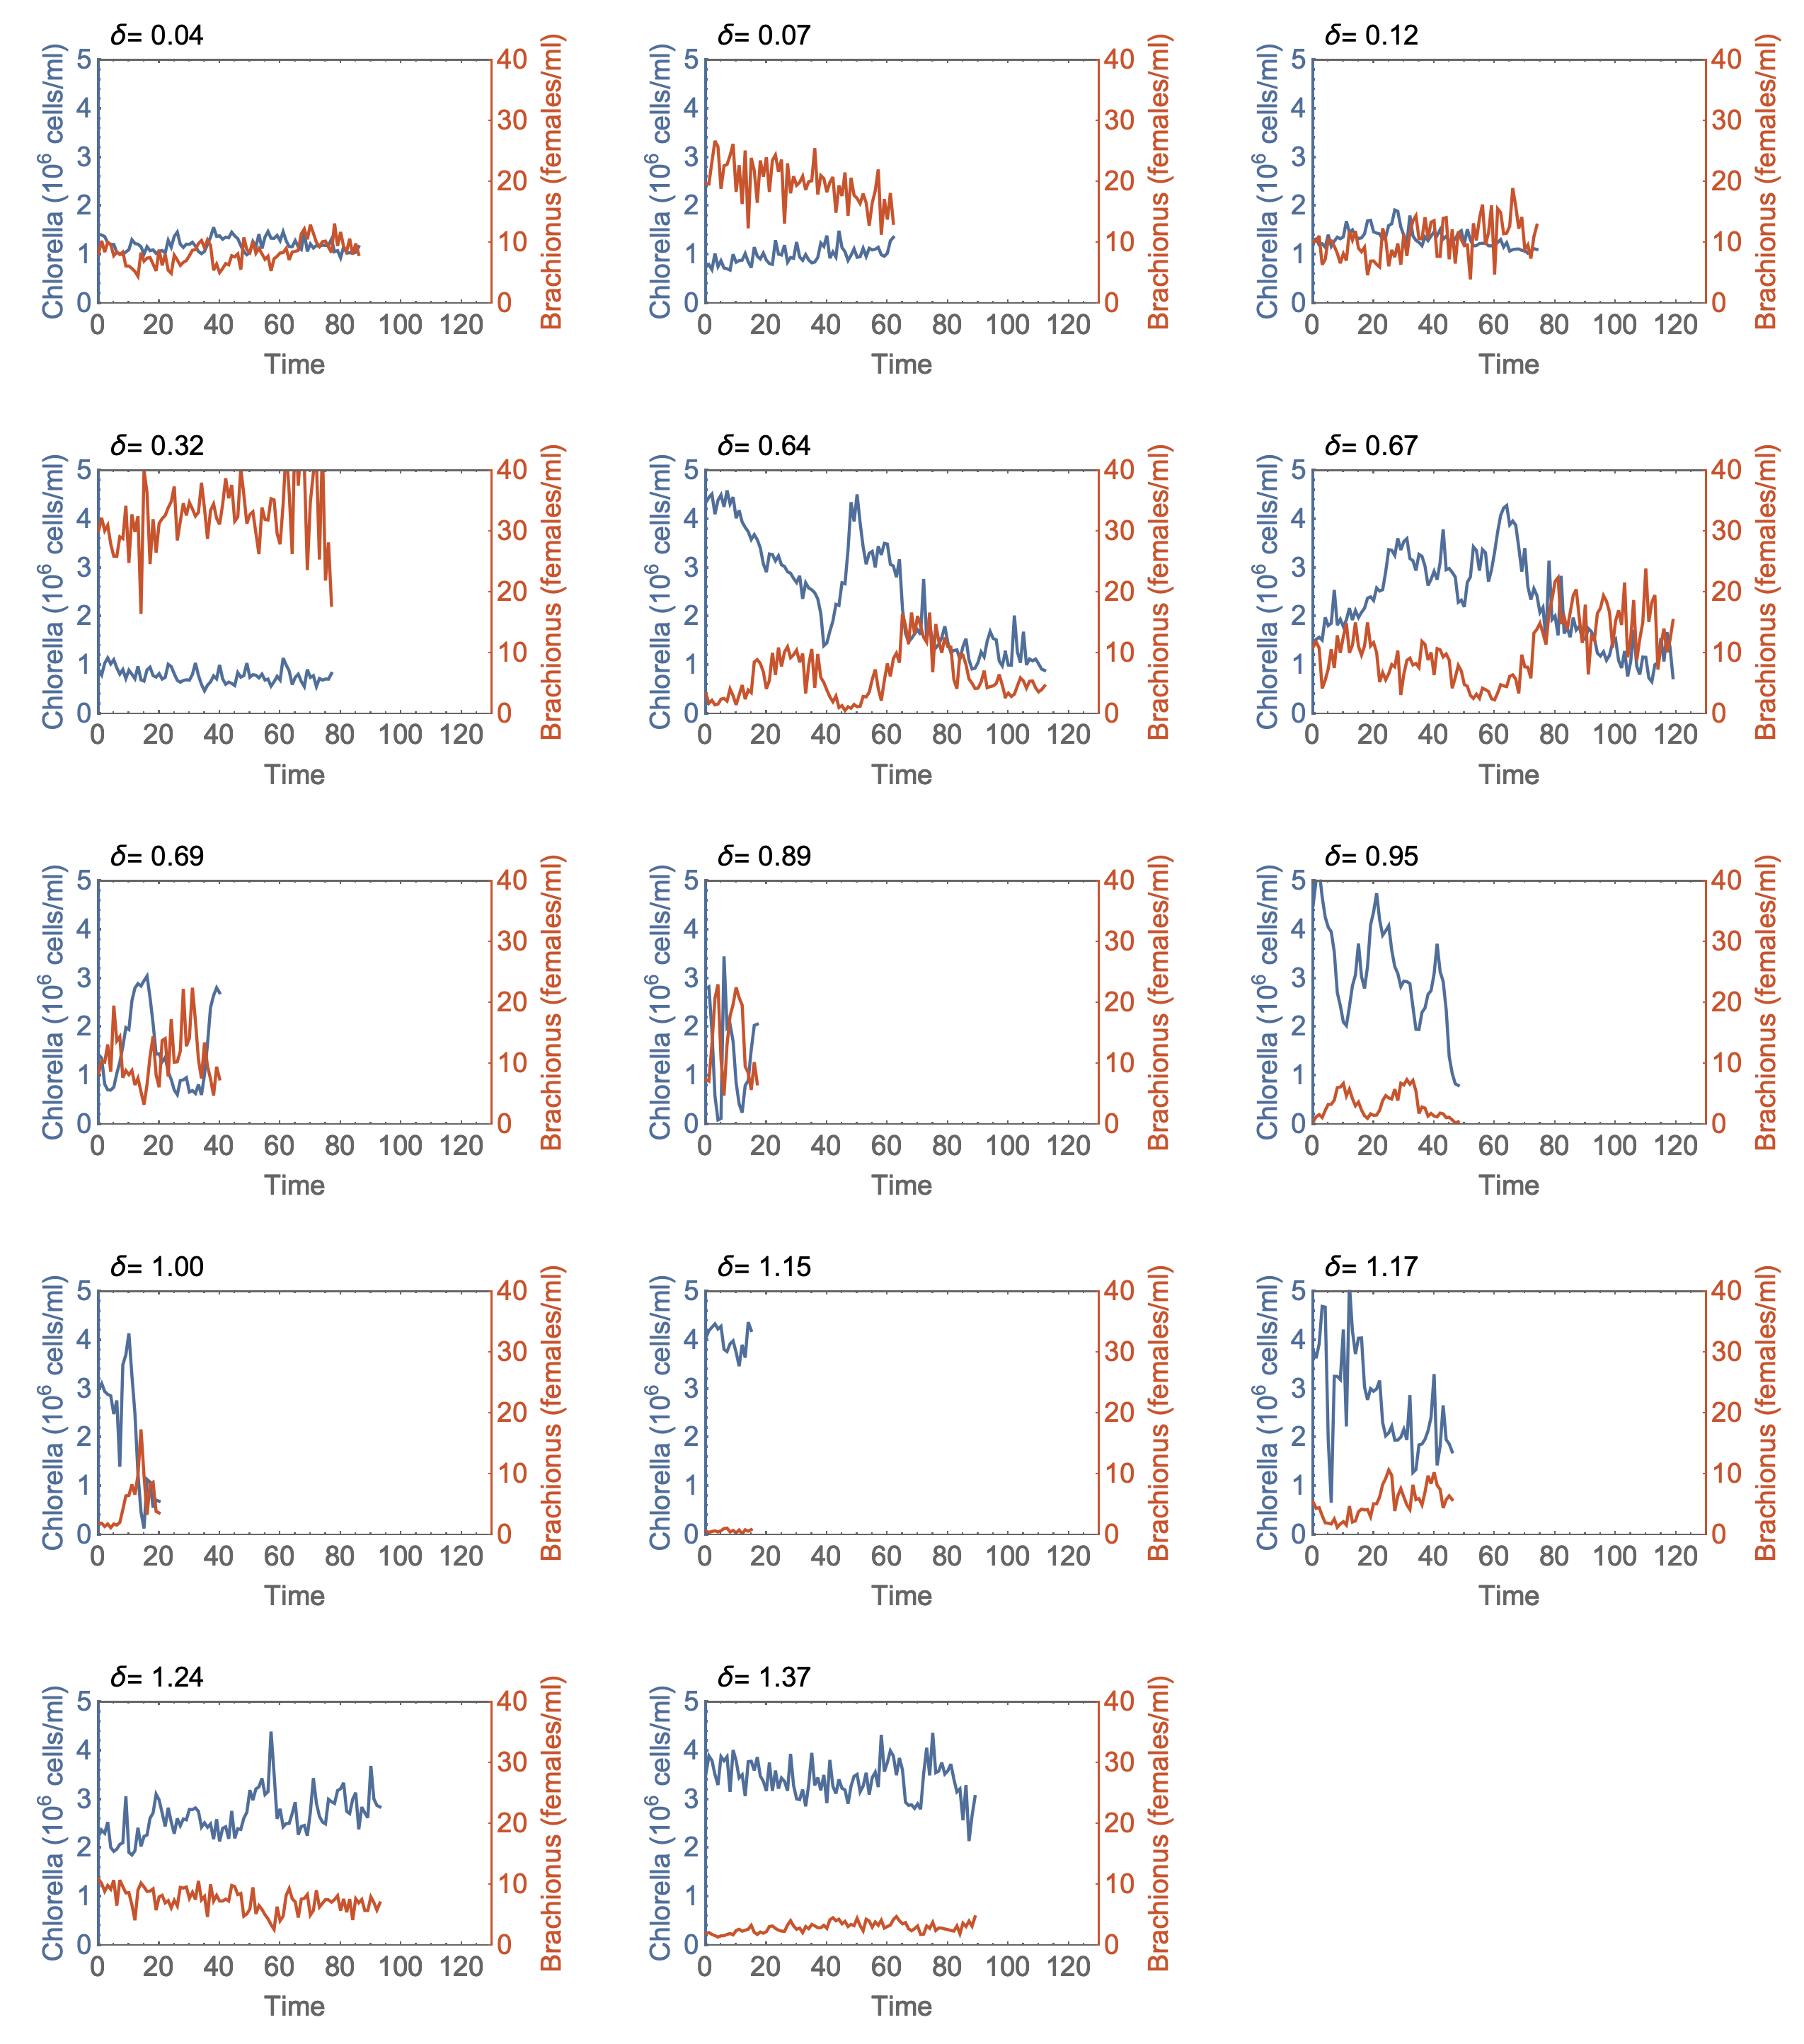
\includegraphics[width=\textwidth]{empirical_tseries.png}
\vspace{0.4cm}
\caption{\textbf{Predator-prey trajectories from chemostat experiments (from Fussmann et al\cite{fussmann00}).} Time-series data of the prey species (\textit{Chlorella}, blue) and the predator species (\textit{Brachionus}, red) from chemostat experiments run at different dilution rates ($\delta$). The sampling frequency is one measurement per day. A Hopf bifurcation was conjectured to occur in the range $0.32<\delta<0.64$ and at $\delta\approx 1.16$, based on the system's transition from equilibrium to oscillatory behaviour either side of these thresholds.}
\label{fig:fussmann_tseries}
\end{figure}


%---------table: fussmann parameters-----------%
\begin{table}[ht]
\centering
\tabulinesep=0.4mm
\begin{tabu}{l l l}
\hline
Parameter & Definition & Value \\ \hline
%
$\delta$ & dilution rate & (.) per day\\
$N_i$ & nitrogen inflow concentration & $80$ $\mu$mol/liter\\
$b_C$ & maximum birth rate of \textit{Chlorella} & $3.3$ per day \\
$K_C$ & half-saturation constant of \textit{Chlorella} & $4.3$ $\mu$mol/liter \\
$b_B$ & maximum birth rate of \textit{Brachiounus}  & $2.25$ per day \\
$K_B$ & half-saturation constant of \textit{Brachionus} & $15$ $\mu$mol/liter \\
$m$ & mortality of \textit{Brachiounus} & $0.055$ per day \\
$\lambda$ & decay of fecundity of \textit{Brachionus} & $0.4$ per day \\
$\epsilon$ & assimilation efficiency of \textit{Brachionus} & $0.25$ \\
$\eta_C$ & conversion factor $\mu$mol/lit to cells/ml of \textit{Chlorella} & $5\times 10^4$ (cells/ml)($\mu$mol/lit)$^{-1}$ \\
$\eta_B$ & conversion factor $\mu$mol/lit to females/ml of \textit{Brachionus} & $5$ (females/ml)($\mu$mol/lit)$^{-1}$\\
\end{tabu}
\vspace{0.4cm}
\caption{\textbf{Parameter values for the predator-prey model.} Definition and value for each parameter in the predator-prey model given in Eqns. $\eqref{eq:pp1}$-$\eqref{eq:pp4}$. Calibrated by Fussmann et al.\cite{fussmann00} from chemostat experiments or obtained from published sources on \textit{Chlorella} and \textit{Brachionus}.}
\label{tab:fussmann_pars}
\end{table}
%---------------------------

\subsection{Early warning signals in the model}

Here, we investigate how the EWS behave in the predator-prey model, and compare with theoretical expectations. The model possesses several bifurcations in the range of dilution rates considered. With the parameters set to the values displayed in Table \ref{tab:fussmann_pars}, the model exhibits a Hopf bifurcation at $\delta=0.009$ with a period of $T=44.22$ days (H1), a Hopf bifurcation at $\delta = 0.151$ with a period of $T=5.905$ days (H2), a Hopf bifurcation at $\delta = 0.970$ with a period of $T=0.554$ days (H3), and a Transcritical bifurcation at $\delta=1.427$ (T1). The corresponding bifurcation diagram is in Figure \ref{fig:ews_fussmann_model}a. We simulate the model at fixed dilution rates over the range $[0,1.6]$ to investigate the behaviour of each EWS in the vicinity of the bifurcations. After a burn-in period of 500 time units to remove transient dynamics, we measure each EWS statistic over the following 4000 time units. The behaviour of some of the EWS considered is shown in Figure \ref{fig:ews_fussmann_model}b-f.

Variance as an EWS behaves as expected. As the dilution rate approaches each of the three Hopf bifurcations from the neighbouring equilibrium state, the variance of the system dynamics increases, consistent with theory. The variance is maximal in the oscillatory regime between H2 and H3 since oscillations are not filtered out by the smoothing of the time-series. Near the Transcritical bifurcation T1, there is an increase in variance from the right and the left, although this increase occurs relatively late (close to the bifurcation), and is a very slight change in magnitude.



%----- Figure: EWS of model--------
\begin{figure}[H]
\centering
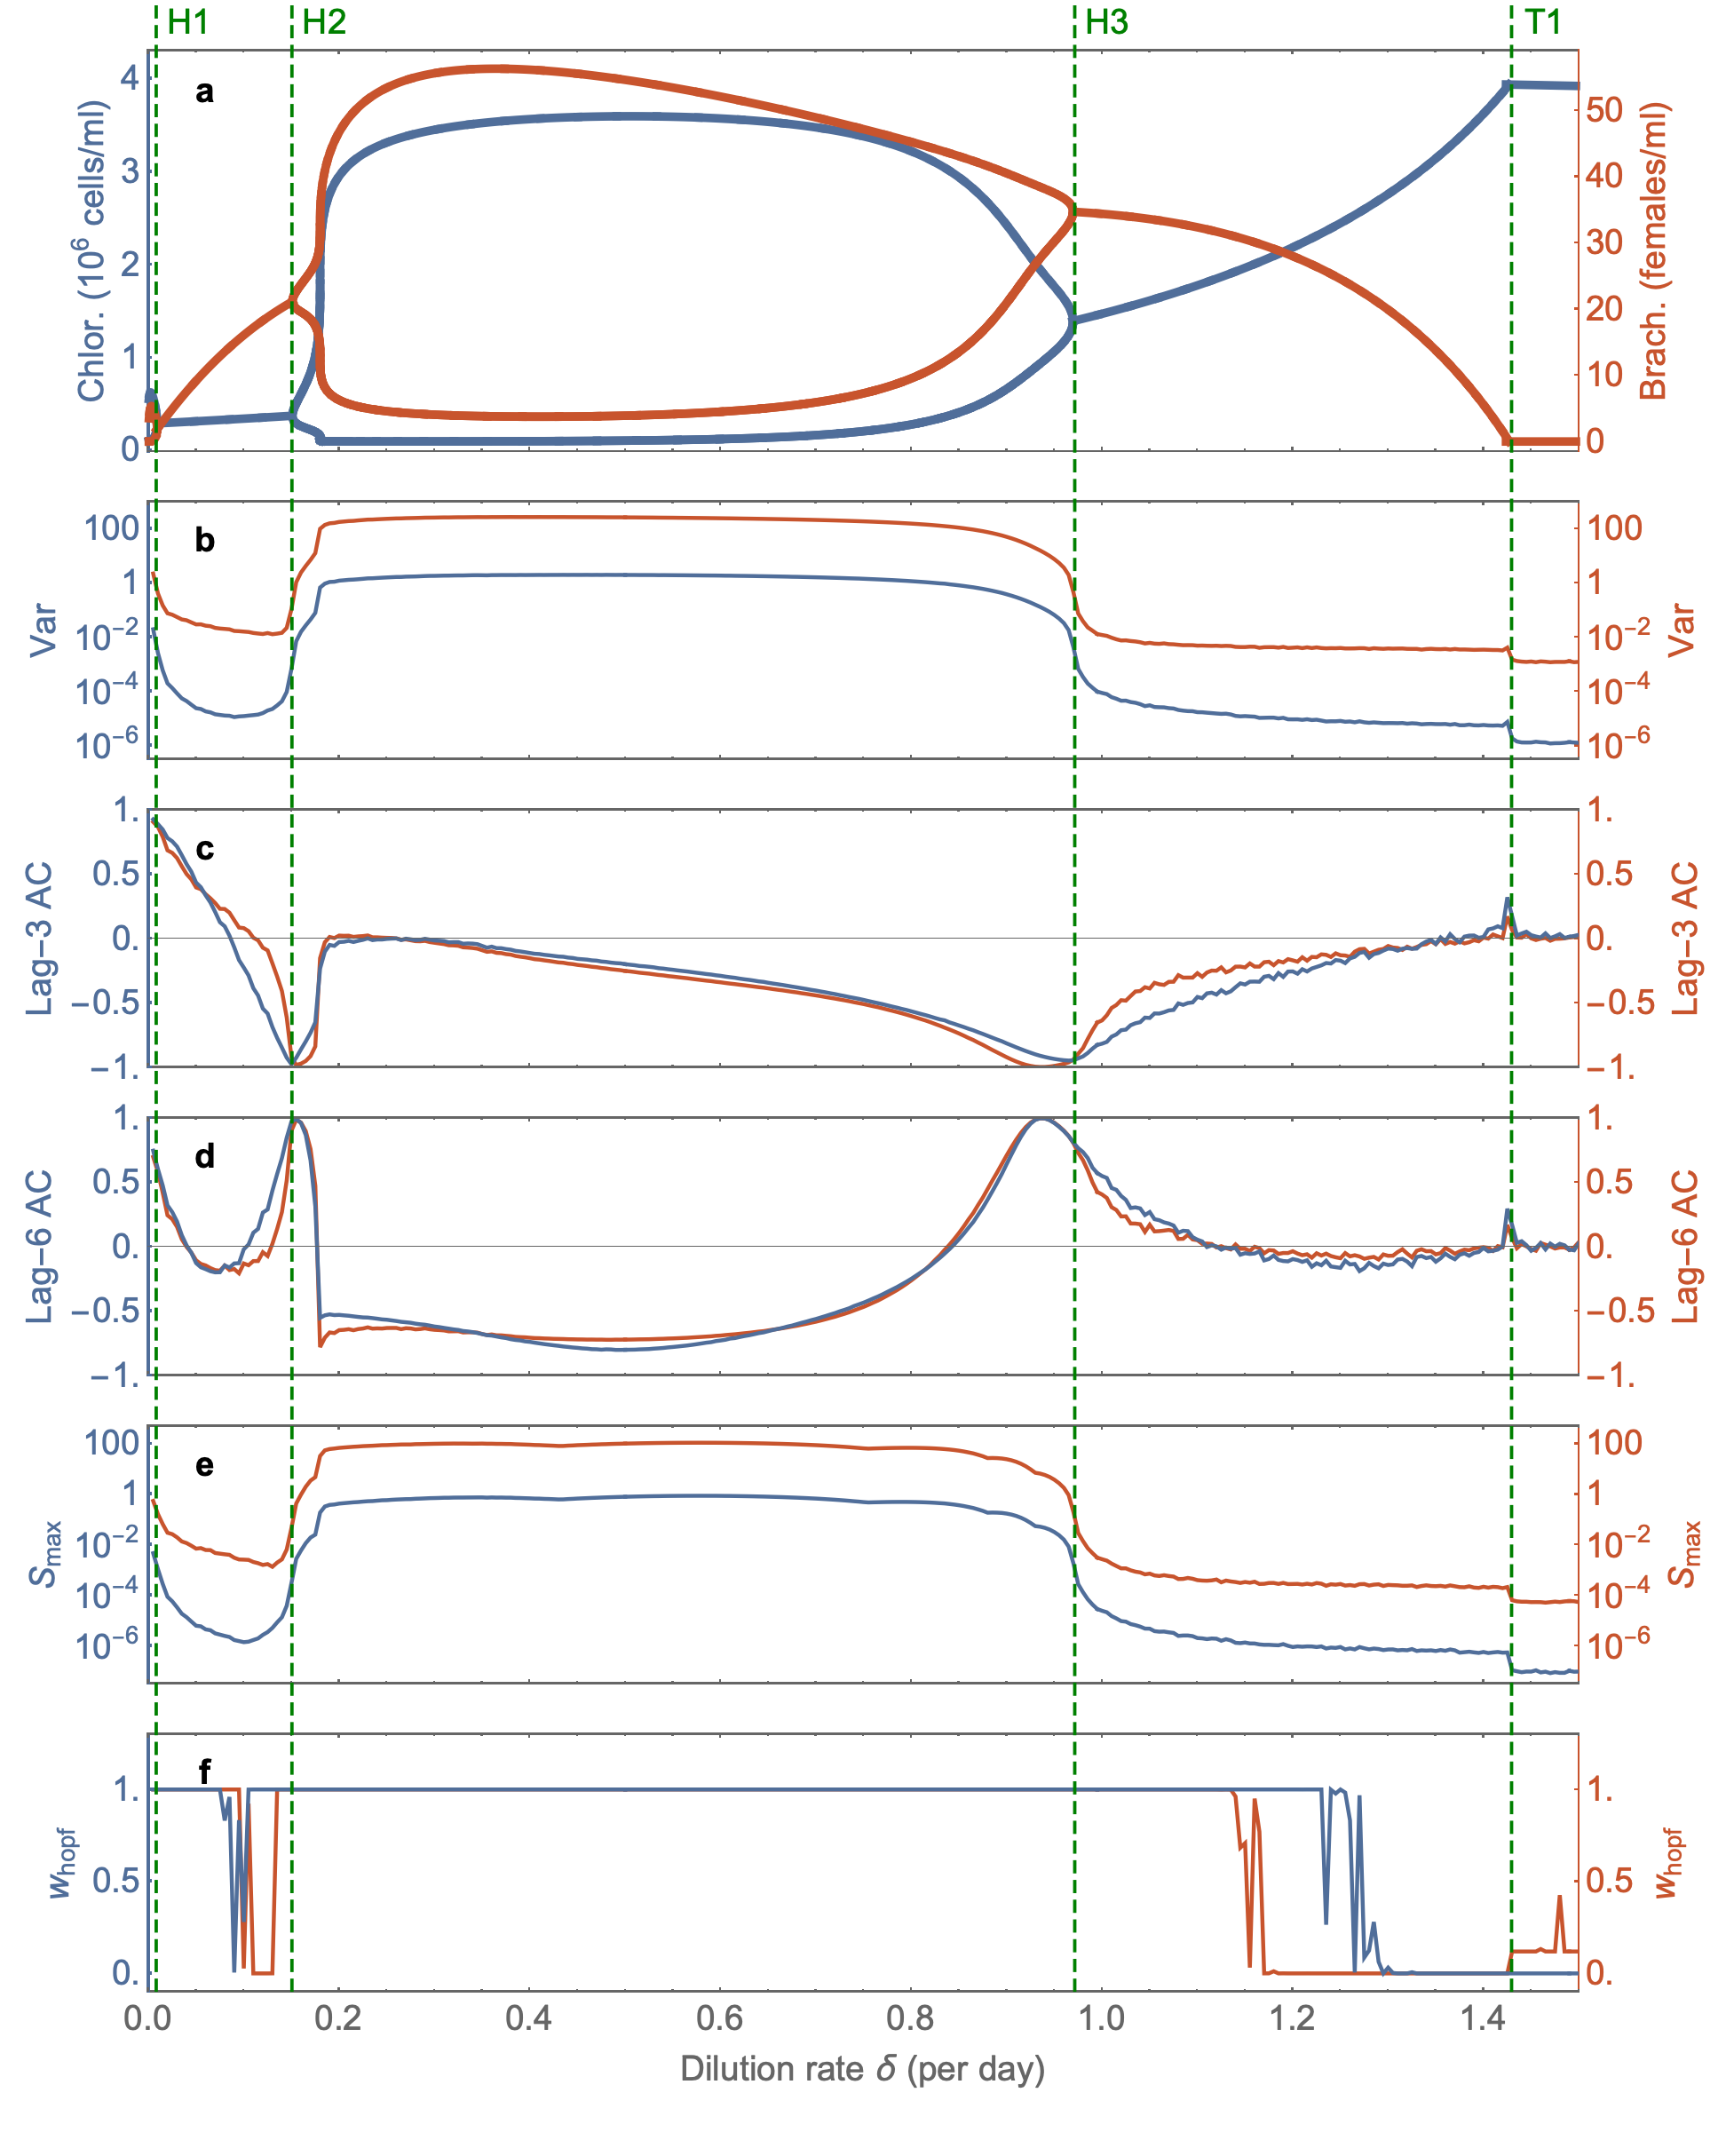
\includegraphics[width=0.9\textwidth]{ews_model.png}
\vspace{0.4cm}
\caption{\textbf{EWS in stationary model simulations.} For fixed dilution rates spaced 0.005 apart, we simulate the model for 4500 time units allowing for a burn-in period of 500 time units to remove any transient behaviour. EWS are then computed on the remaining time-series data. \textbf{a.} Bifurcation diagram showing stable states and extreme points of limit cycles for the prey (\textit{Chlorella}, blue) and the predator (\textit{Brachionus}, red). \textbf{b.} Variance. \textbf{c-d.} Lag-3 and lag-6 autocorrelation. \textbf{e.} Peak in the power spectrum. \textbf{f.} Hopf AIC weight. Green dashed lines mark the Hopf bifurcations (H1, H2, H3) and the Transcritical bifurcation (T1). EWS are computed as in Methods.} 
\label{fig:ews_fussmann_model}
\end{figure}
%----------------------

Autocorrelation also behaves as expected, and we have displayed lag times of 3 and 6 as they exemplify the contrasting behaviour that autocorrelation can exhibit depending on the chosen lag time. Recall that the analytical form for the autocorrelation in the vicinity of a Hopf bifurcation has a multiplicative factor of $\cos(2\pi\tau/T)$ (Section \ref{sec:derivations}), where $\tau$ is the lag time and $T$ is the period of oscillations at the Hopf bifurcation. The other factor approaches one as the Hopf bifurcation is approached, just like the case for the Fold bifurcation. Since the period at H2 is approximately 6, this multiplicative factor will be negative for $\tau=3$ (resulting in decreasing autocorrelation) and positive for $\tau=6$ (resulting in increasing autocorrelation). Note that for certain lag times ($\tau=T/4, 3T/4$) this factor is zero, in which case autocorrelation does not serve as an EWS. In general, we do not know the period at a Hopf bifurcation in advance, and so choosing an appropriate lag time is difficult. The power spectrum is not hindered by this uncertainty, since it captures the equivalent information to autocorrelation at every lag time\cite{box15}.

The peak in the power spectrum ($S_{\text{max}}$) behaves very similarly to the variance. It as at least as good as Variance at signalling bifurcations. Preceding H2 it actually provides earlier warning as can be seen in Figure \ref{fig:ews_fussmann_model_H2}, which zooms in on the preceding dynamics.

The Hopf AIC weight ($w_{\text{hopf}}$) correctly signals which bifurcations are Hopf, and which are not. (Preceding H1-H3 it attains 1 the value 1, and preceding T1 it attains the value 0). The metric appears to be quite late in recognising a Hopf bifurcation in the Brachionus time-series preceding H2. Zooming in on this area (Figure \ref{fig:ews_fussmann_model_H2}), we see that the signalling of $w_{\text{hopf}}$ aligns with the moment when variance and $S_{\text{max}}$ begin to increase.





% Figure: EWS of model - zoom in on H2
\begin{figure}[H]
\centering
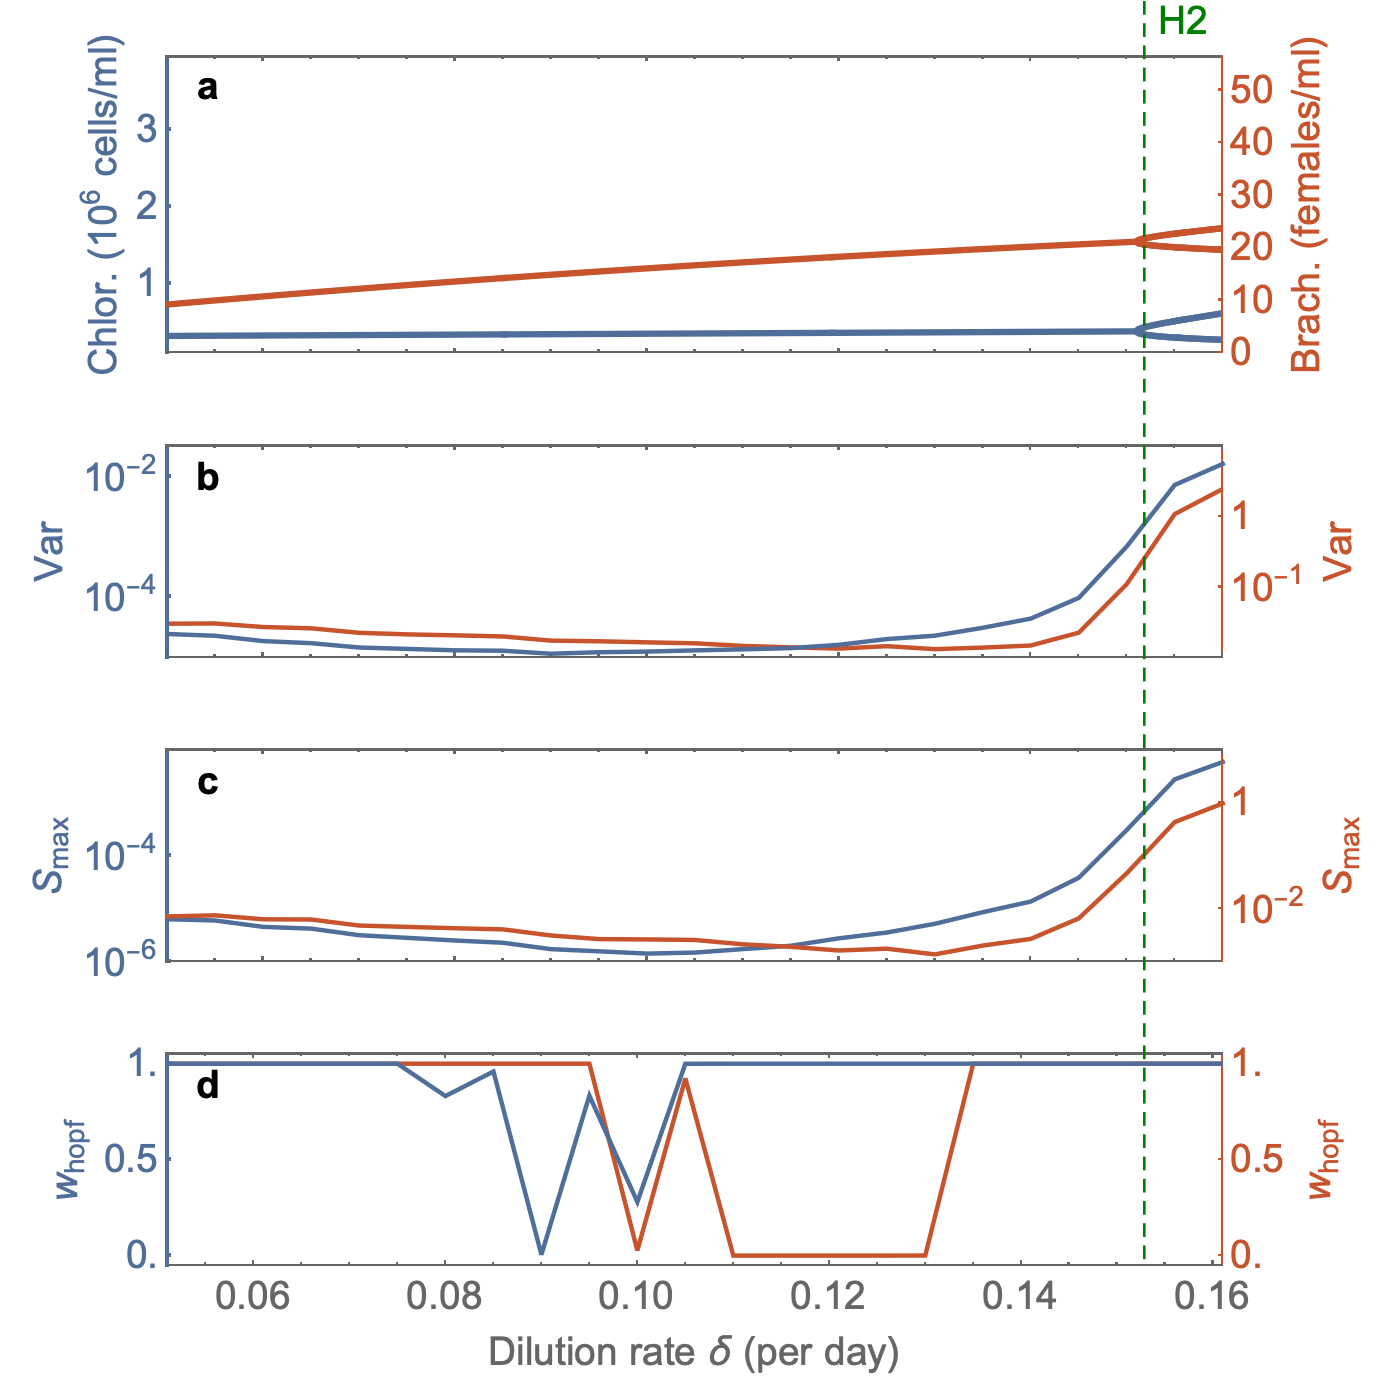
\includegraphics[width=0.75\textwidth]{ews_modelH2.png}
\vspace{0.4cm}
\caption{\textbf{EWS in stationary model simulations - zoom in on H2.} As in Figure \ref{fig:ews_fussmann_model} except zoomed in on the dynamics preceding H2. $S_{\text{max}}$ does at least as well as variance in signalling the upcoming bifurcation, performing better than variance with the Brachionus time-series. The Hopf AIC weight registers the type of bifurcation for each species once $S_{\text{max}}$ begins to increase.} 
\label{fig:ews_fussmann_model_H2}
\end{figure}





%-------EWS in experiments----------------
\subsection{Early warning signals in the experiments}

From the experimental data, the authors found that the first Hopf bifurcation lies in the region $0.32<\delta<0.64$, and the second Hopf bifurcation lies at $\delta\approx 1.16$. As with most simple models, the model does well at describing the system's qualitative dynamics, but it does not accurately determine certain quantitative features such as the location of the bifurcation points and the period of oscillations. This could be due to subtle inaccuracies in the parameter estimation, or additional mechanisms not represented in the model. Figure \ref{fig:fussmann_ews}a shows the bifurcation diagram of the model and the estimated regions where the Hopf bifurcation occurs in the real system (shaded grey), which do not line up. Inaccuracies such as these are inevitable in models of complex systems, emphasising the importance of complementing parameterised models with time-series analysis to improve our ability in forecasting upcoming bifurcations.

For each chemostat time-series (Figure \ref{fig:fussmann_tseries}) with more than 25 data points, we compute the EWS metrics as detailed in Section \ref{sec:ews_computation}. (Since we use a Hamming window size of 40, we require at least 40 data points in the time-series. It is also recommended for autocorrelation that there are at least 50 data points \cite{box15}.) The EWS metrics for each time-series are shown in Figure \ref{fig:fussmann_ews}. Note as with the model simulations, $S_{\text{max}}$ performs at least as well as variance, showing a larger relative change in magnitude. Lag-1 autocorrelation appears to provide a weak signal of increasing prior to the Hopf bifurcations (an increase is expected in theory since the period of oscillations in the experiments is about 20 days). The Hopf AIC weight correctly identifies the Hopf bifurcations that correspond to H1, H2 and H3 in the model. For the Chlorella time-series, it is able to provide this information well in advance of the bifurcations.

The spectral EWS for a selection of the experiments with particularly long time-series are shown in Figure \ref{fig:fussmann_ews_pspecs} along with their power spectra. Note that even in the equilibrium regimes, one can observe a power spectrum characteristic of a Hopf bifurcation. Moreover, monitoring the power spectrum gives an idea as to the frequency to expect at the Hopf bifurcation. This is demonstrated in the Chlorella time-series leading up to the Hopf bifurcation at $\delta\approx 1.16$. Suppose we have no knowledge of the bifurcation structure, and we observe the time-series at $\delta = 1.37$. We see there is a dominant frequency in the power spectrum - something to note in case of a sudden increase in $S_{\text{max}}$or variance. Suppose the dilution rate begins decreasing - we would observe time-series more akin to that of $\delta=1.17$, where $S_{\text{max}}$ has dramatically increased. We therefore expect an upcoming bifurcation. Since $w_{\text{hopf}}=1$ we can say with a high probability that this is an incoming Hopf bifurcation, and the power spectrum tells us that we can expect a frequency of $\omega\approx0.3$. This corresponds to a period of about 20 days, which is roughly the period of oscillations observed during the oscillatory phase of the dynamics ($\delta=0.69,0.95$). So not only can the power spectrum, classify the upcoming bifurcation as Hopf, but is can put a value on the frequency of oscillations to expect at the Hopf bifurcation.

The full set of power spectra from the experimental time-series is given in Figures \ref{fig:fussmann_pspec_chlor} and \ref{fig:fussmann_pspec_brach}, along with the AIC fits.


% PUT SOMEWHERE IN METHODS (EWS COMPUTATION FOR EMPIRICAL DATASET)
% For the time-series corresponding to each chemostat setup, we compute the EWS metrics as follows. The time-series is first detrended using a Gaussian filter of bandwidth 30 days to deal with any unintentional drift in the dilution rate. Note that the bandwidth should be chosen small enough to capture slow changes in $\delta$, but large enough so not to filter out the frequencies corresponding to the oscillatory dynamics (which have period approximately 20 days). From the residual dynamics, we then compute the variance (Var), coefficient of variation (C.V.), lag-1 autocorrelation (AC) Hopf AIC weight ($w_h$), Fold AIC weight ($w_f$), peak in the power spectrum ($S_{\text{max}}$) and the coherence factor (CF) using the methods outlines in Appendix \ref{sec:ews_computation}. We do not use a rolling window for these computations as we are simply interested in the EWS metrics over the time-series as whole (the bifurcation parameter is fixed). The power spectrum is computed using a Hamming window of length $40$ data points with an overlap of $50\%$. The power spectrum, and EWS metrics for each empirical time-series is shown in Figure \ref{fig:fussmann_ews_spectra_full}. 



% Figure: EWS of empirical predator-prey as a series
\begin{figure}[H]
\centering
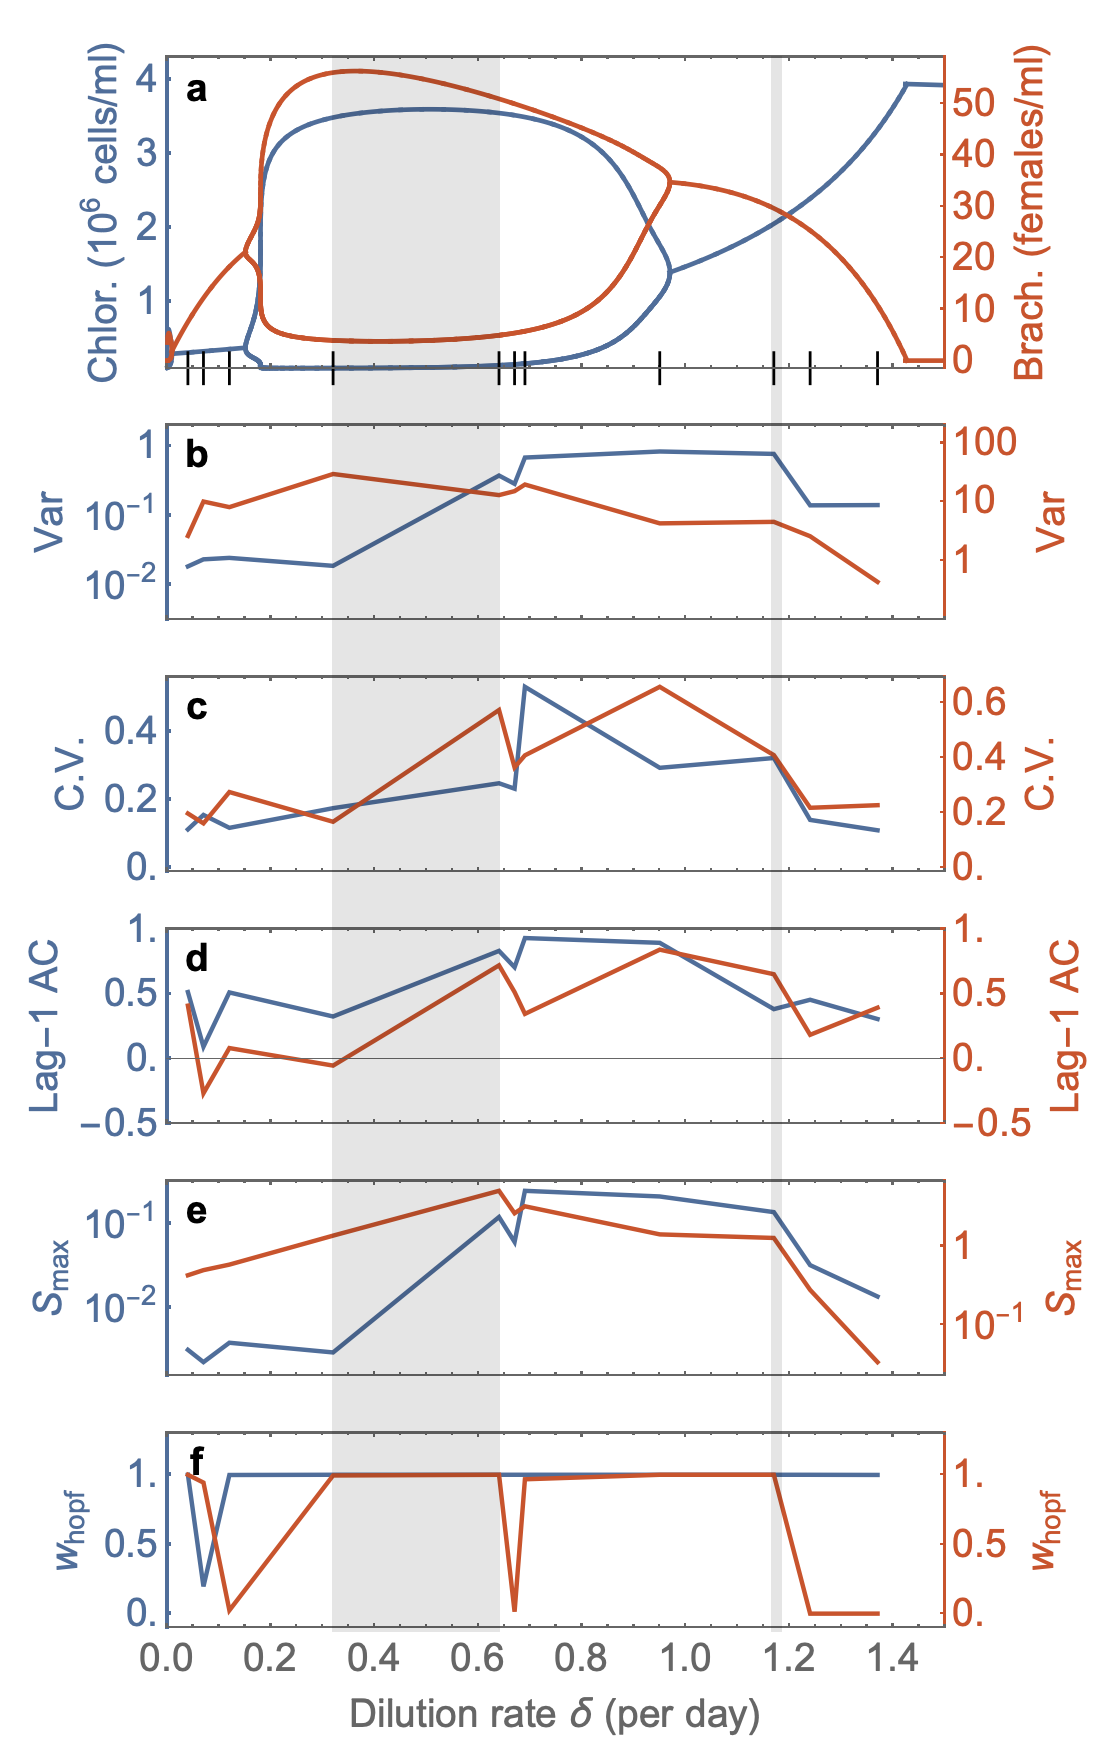
\includegraphics[width=0.5\textwidth]{ews_series_log.png}
\vspace{0.4cm}
\caption{\textbf{EWS in the empirical predator-prey system.} \textbf{a.} Bifurcation diagram of the model system showing the maxima and minima of the the prey (\textit{Chlorella}, blue line) and the predator (\textit{Brachionus}, red line). Grey regions mark where Hopf bifurcations occur in the experimental system. Black dashes mark the fixed dilution rates used in chemostat experiments. We only consider the experiments that have a time-series of 25 points or more in length forcing us to remove three experiments from the dataset. \textbf{b-d.} Standard EWS including variance (Var), coefficient of variation (C.V.) and lag-1 autocorrelation (AC), evaluated for each time-series and plotted at the corresponding dilution rate. \textbf{e-f.} Spectrum-based EWS including the peak in the power spectrum ($S_{\text{max}}$) and the Hopf AIC weight ($w_{\text{hopf}}$). Note that both variance and $S_{\text{max}}$ are plotted on a log scale. EWS are computed as in Methods.}
\label{fig:fussmann_ews}
\end{figure}


% Figure: spectral EWS and bifurcation diagram of empirical predator-prey system
\begin{figure}[H]
\centering
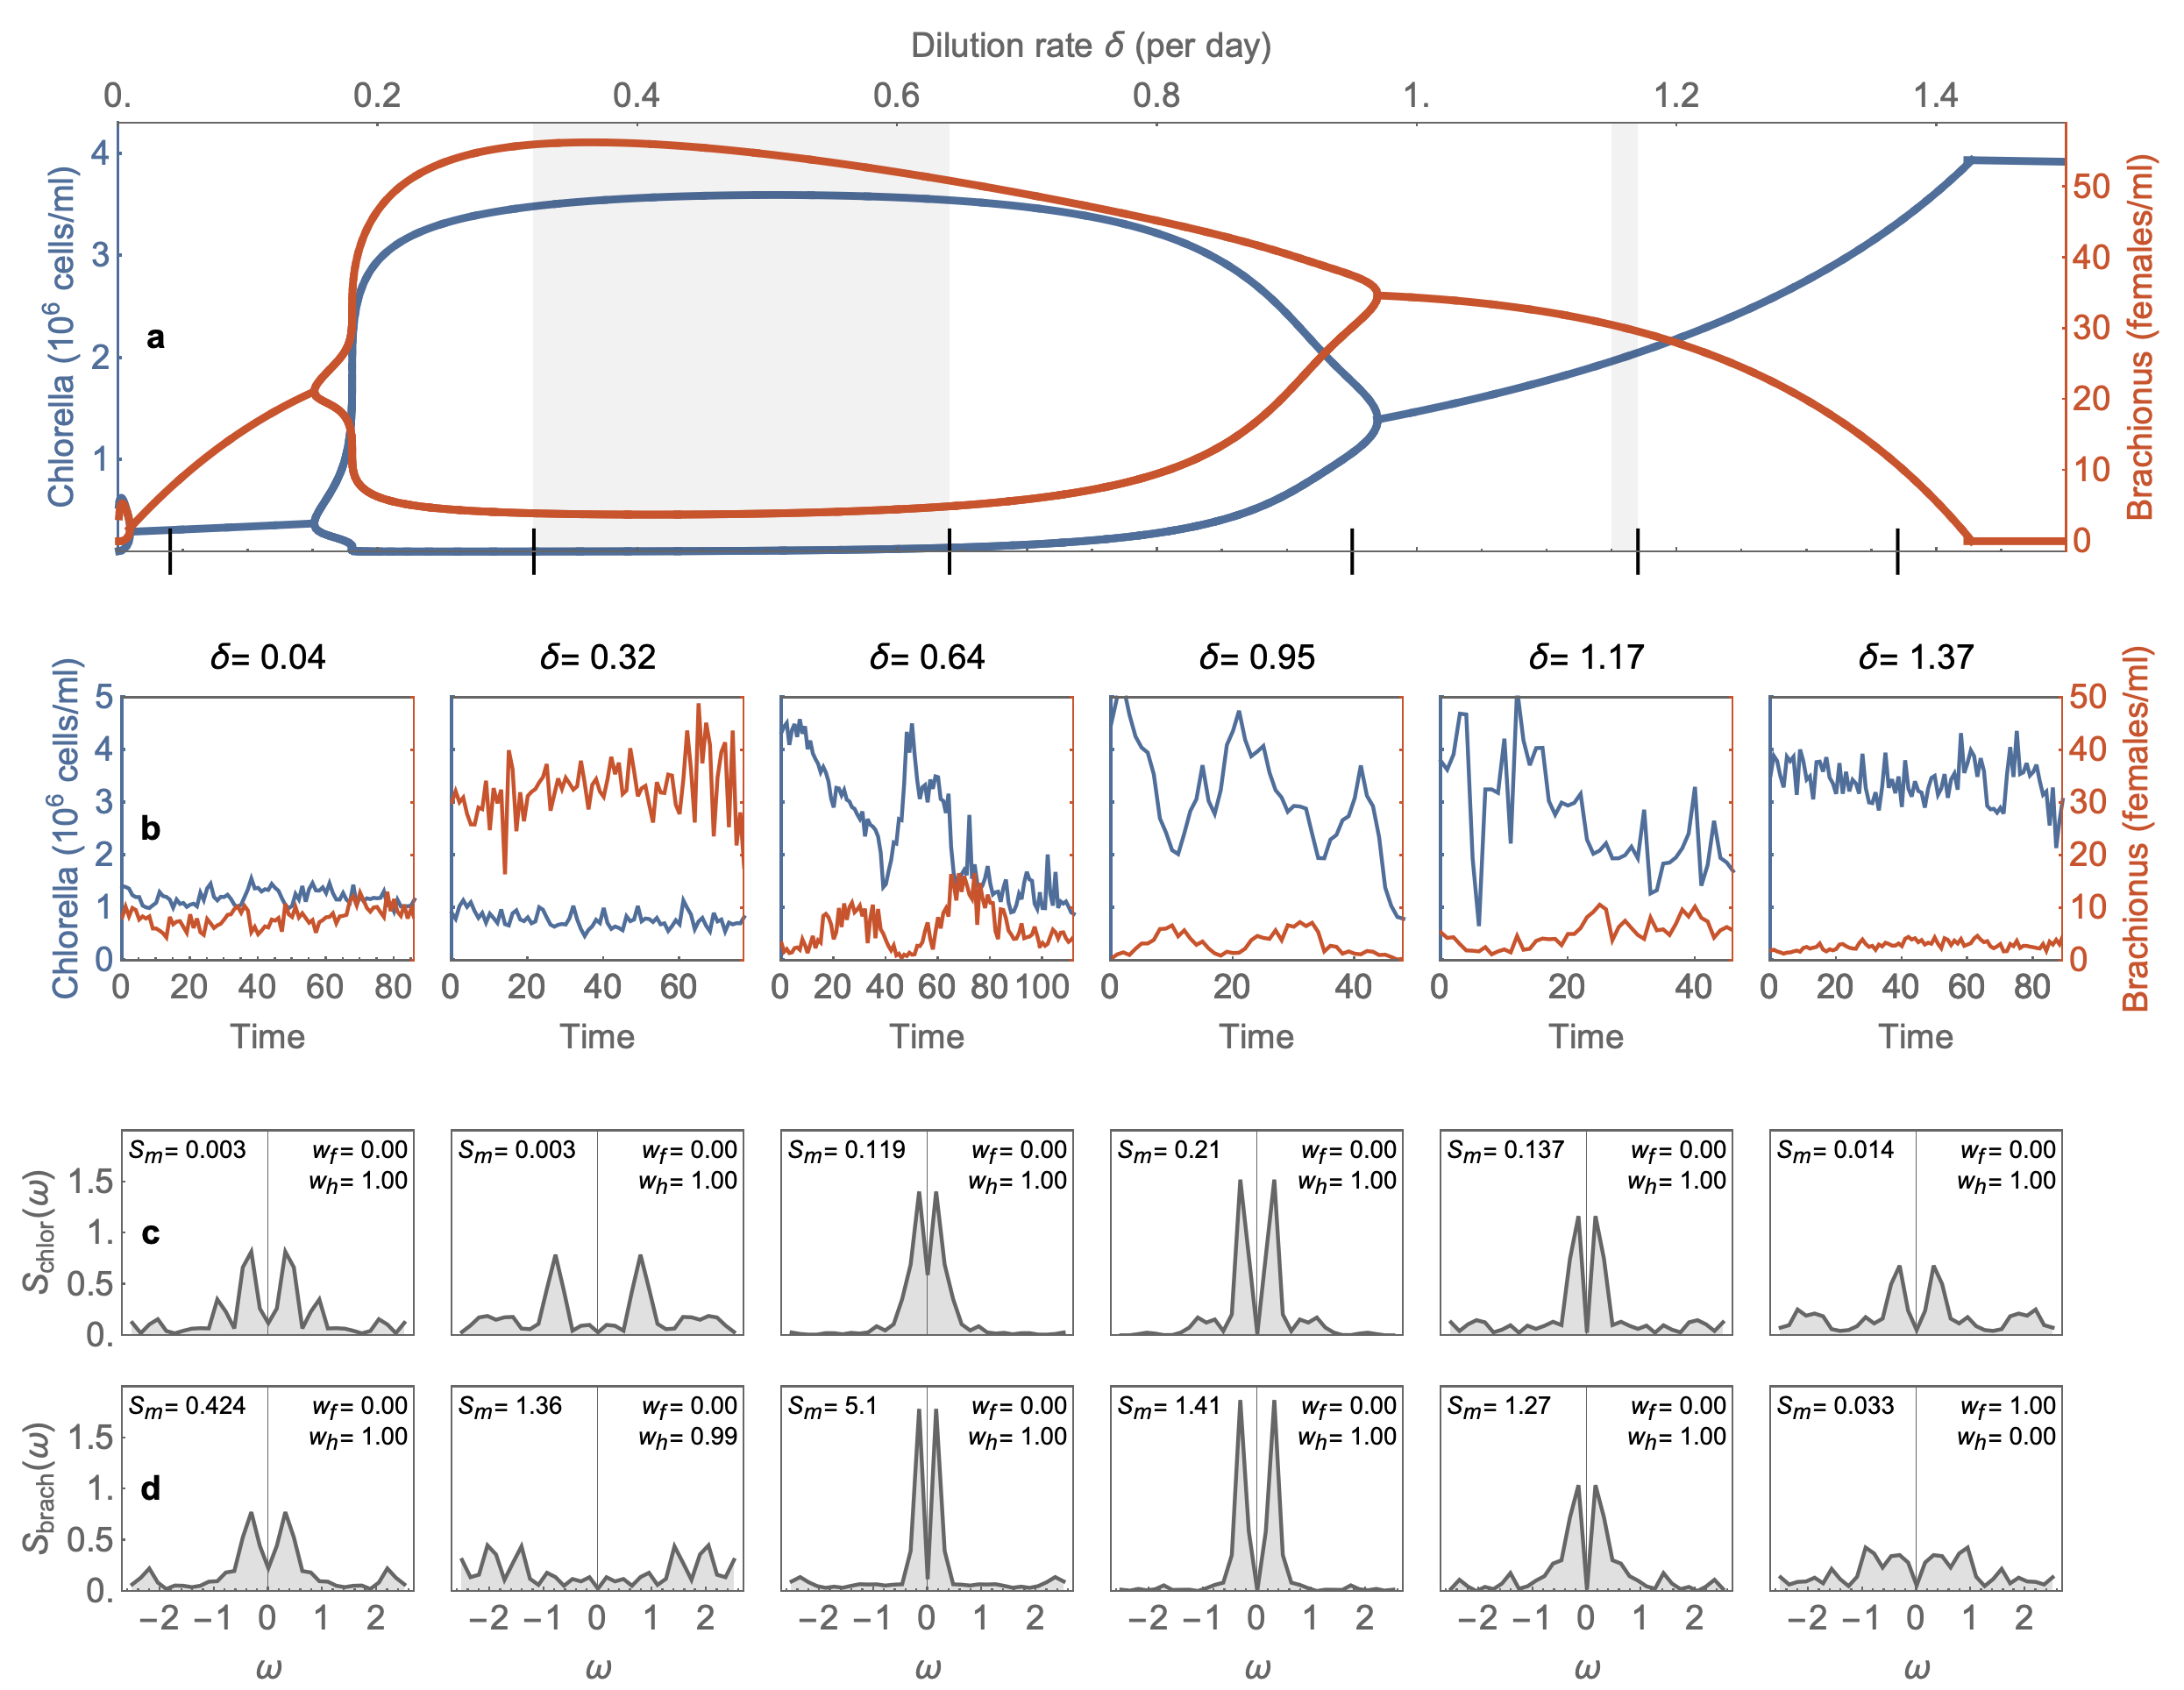
\includegraphics[width=\textwidth]{fussmann_ews_pspecs.png}
\vspace{0.4cm}
\caption{\textbf{Spectral EWS for the empirical predator-prey system.} \textbf{a.} Bifurcation diagram of the model system showing equilibria / extreme points of limit cycles for the prey (\textit{Chlorella}, blue) and predator (\textit{Brachionus}, red). The two grey regions mark where the two Hopf bifurcations occur in the empirical system. Black dashes mark the dilution rates shown in b. \textbf{b.} Empirical time-series data from chemostats with the given dilution rate ($\delta$). \textbf{c-d,} Normalised power spectra of the time-series data in b for \textit{Chlorella} and \textit{Brachionus} respectively. Data insets give the peak power ($S_{\text{max}}$), the Fold AIC weight ($w_{\text{f}}$) and the Hopf AIC weight ($w_{\text{h}}$).}
\label{fig:fussmann_ews_pspecs}
\end{figure}









% Figure: Power spectra of Chlorella
\begin{figure}[H]
\centering
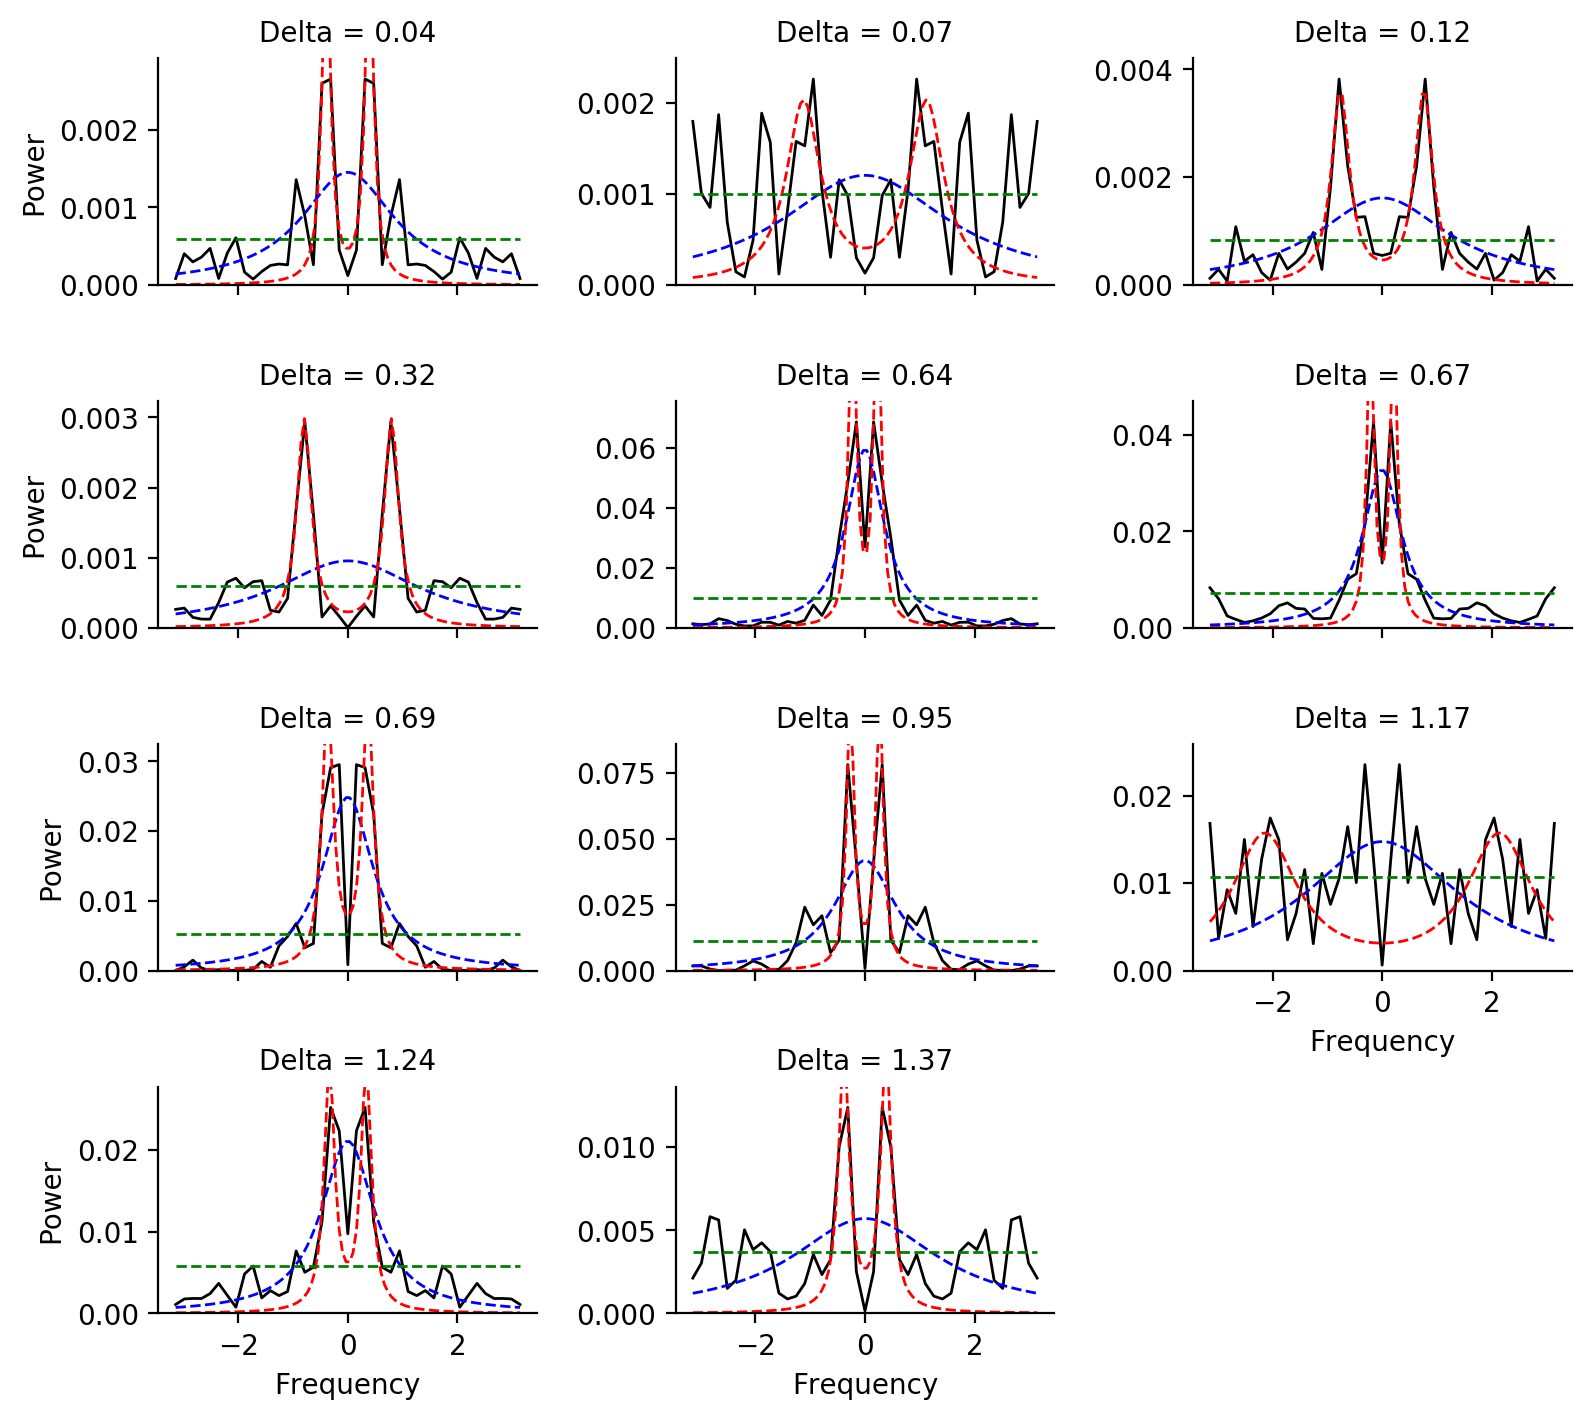
\includegraphics[width=\textwidth]{pspec_grid_chlor.png}
\vspace{0.4cm}
\caption{\textbf{Power spectra of the Chlorella time-series at each dilution rate ($\delta$).} The power spectrum (black) is computed using Welch's method with a Hamming window of length 40 days and a 50\% offset. After imposing a frequency cutoff of $\omega_{\text{cutoff}}=0.8$, the analytical forms $S_{\text{fold}}$ (blue), $S_{\text{hopf}}$ (red) and $S_{\text{null}}$ (green) are fit to the power spectrum to obtain the AIC weights $w_f$, $w_h$ and $w_n$, which are an indication of which fit best explains the data.}
\label{fig:fussmann_pspec_chlor}
\end{figure}



% Figure: Power spectra of Brachiounus
\begin{figure}[H]
\centering
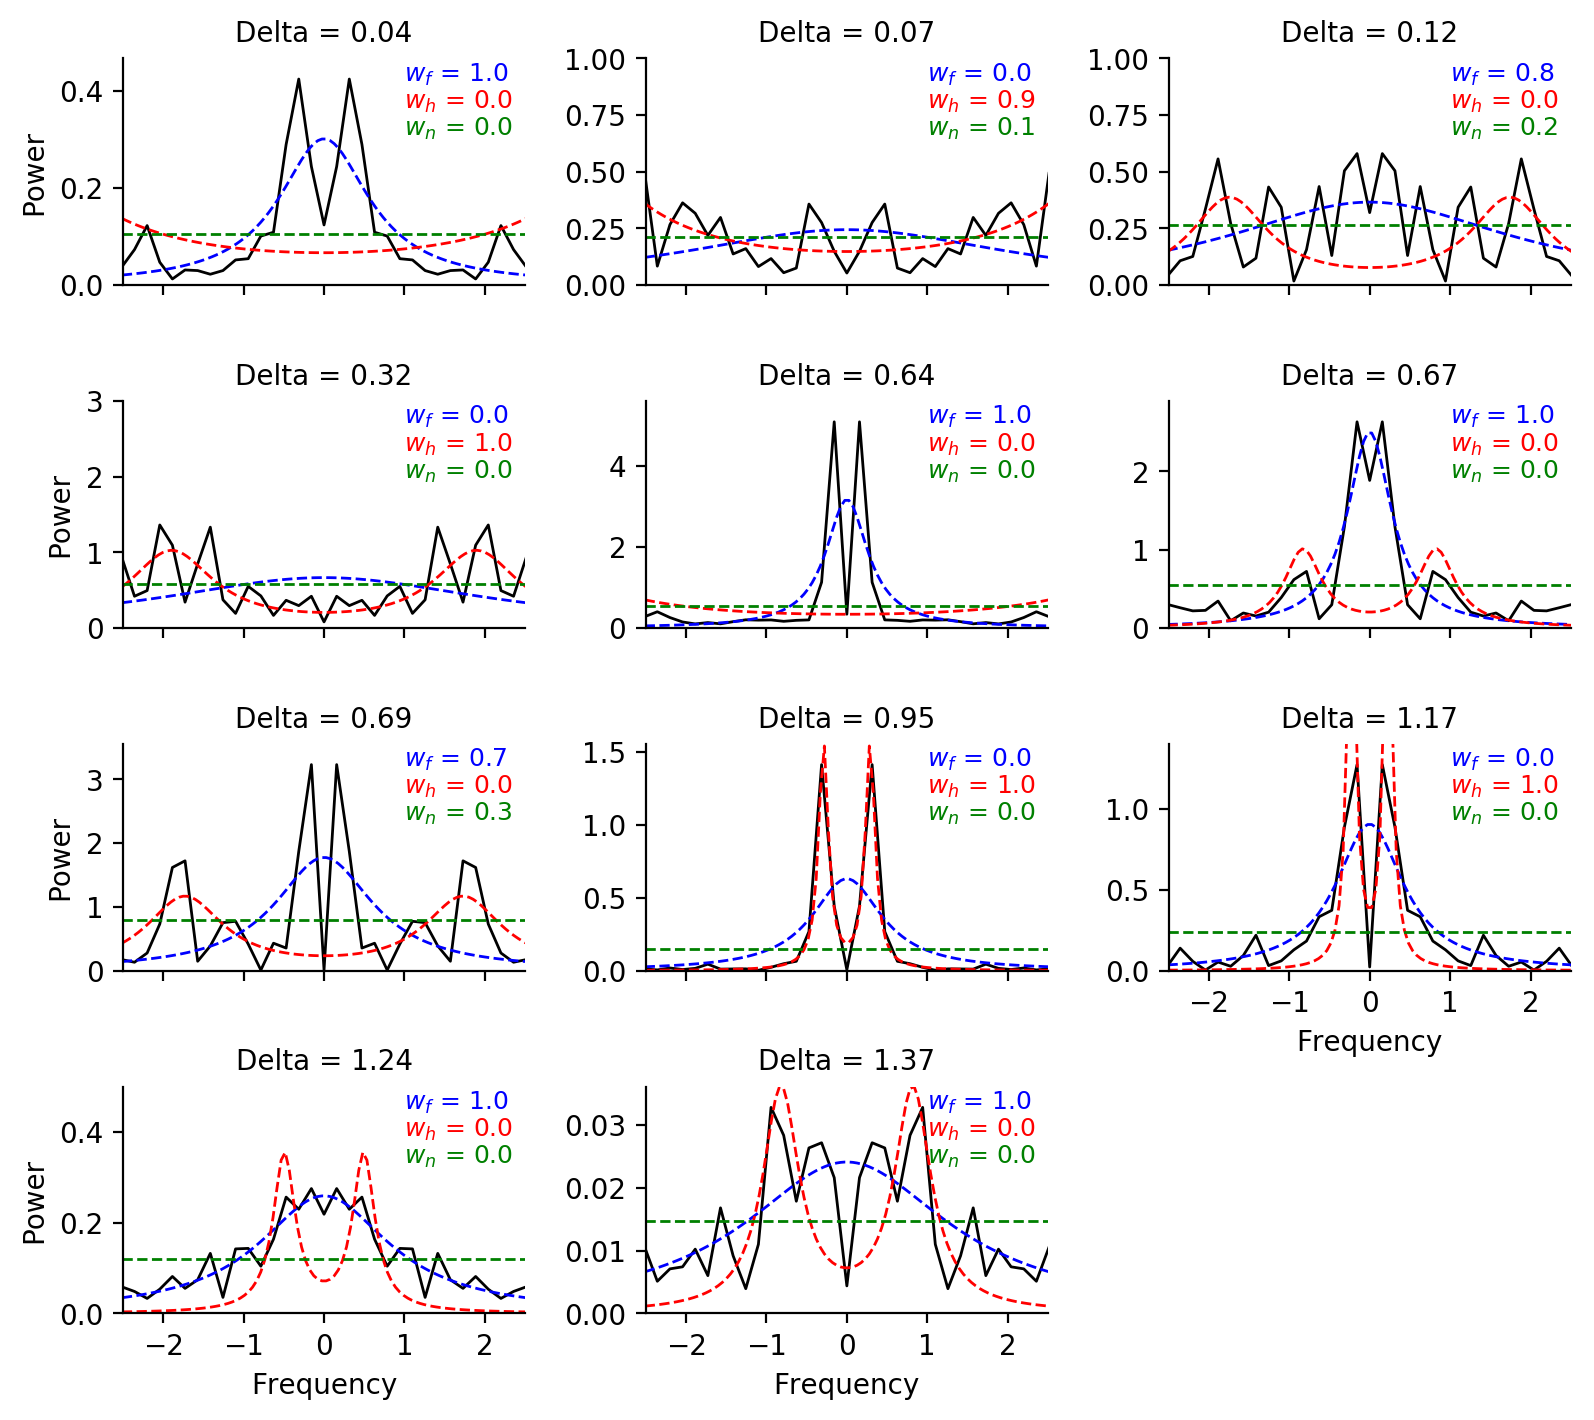
\includegraphics[width=\textwidth]{pspec_grid_brach.png}
\vspace{0.4cm}
\caption{\textbf{Power spectra of the Brachiounus time-series at each dilution rate ($\delta$).} The power spectrum (black) is computed using Welch's method with a Hamming window of length 40 days and a 50\% offset. After imposing a frequency cutoff of $\omega_{\text{cutoff}}=0.8$, the analytical forms $S_{\text{fold}}$ (blue), $S_{\text{hopf}}$ (red) and $S_{\text{null}}$ (green) are fit to the power spectrum to obtain the AIC weights $w_f$, $w_h$ and $w_n$, which are an indication of which fit best explains the data.}
\label{fig:fussmann_pspec_brach}
\end{figure}

\pagebreak


% Insert bibliography
\pagebreak
\bibliographystyle{unsrt}
\bibliography{../../../bibliographies/critical_transitions.bib}





\end{document}